
% Licensed to the Apache Software Foundation (ASF) under one or more
% contributor license agreements.  See the NOTICE file distributed with
% this work for additional information regarding copyright ownership.
% The ASF licenses this file to You under the Apache License, Version 2.0
% (the "License"); you may not use this file except in compliance with
% the License.  You may obtain a copy of the License at
%
%     http://www.apache.org/licenses/LICENSE-2.0
%
% Unless required by applicable law or agreed to in writing, software
% distributed under the License is distributed on an "AS IS" BASIS,
% WITHOUT WARRANTIES OR CONDITIONS OF ANY KIND, either express or implied.
% See the License for the specific language governing permissions and
% limitations under the License.

\chapter{Accumulo Design}

\section{Data Model}

Accumulo provides a richer data model than simple key-value stores, but is not a
fully relational database. Data is represented as key-value pairs, where the key and
value are comprised of the following elements:

\begin{center}
$\begin{array}{|c|c|c|c|c|c|} \hline
\multicolumn{5}{|c|}{\mbox{Key}} & \multirow{3}{*}{\mbox{Value}}\\ \cline{1-5}
\multirow{2}{*}{\mbox{Row ID}}& \multicolumn{3}{|c|}{\mbox{Column}} & \multirow{2}{*}{\mbox{Timestamp}} & \\ \cline{2-4}
& \mbox{Family} & \mbox{Qualifier} & \mbox{Visibility} & & \\ \hline
\end{array}$
\end{center}

All elements of the Key and the Value are represented as byte arrays except for
Timestamp, which is a Long. Accumulo sorts keys by element and lexicographically
in ascending order. Timestamps are sorted in descending order so that later
versions of the same Key appear first in a sequential scan. Tables consist of a set of
sorted key-value pairs.

\section{Architecture}

Accumulo is a distributed data storage and retrieval system and as such consists of
several architectural components, some of which run on many individual servers.
Much of the work Accumulo does involves maintaining certain properties of the
data, such as organization, availability, and integrity, across many commodity-class
machines.

\section{Components}

An instance of Accumulo includes many TabletServers, one Garbage Collector process, 
one Master server and many Clients.

\subsection{Tablet Server}

The TabletServer manages some subset of all the tablets (partitions of tables). This includes receiving writes from clients, persisting writes to a
write-ahead log, sorting new key-value pairs in memory, periodically
flushing sorted key-value pairs to new files in HDFS, and responding
to reads from clients, forming a merge-sorted view of all keys and
values from all the files it has created and the sorted in-memory
store.

TabletServers also perform recovery of a tablet
that was previously on a server that failed, reapplying any writes
found in the write-ahead log to the tablet.

\subsection{Garbage Collector}

Accumulo processes will share files stored in HDFS.  Periodically, the Garbage
Collector will identify files that are no longer needed by any process, and
delete them.

\subsection{Master}

The Accumulo Master is responsible for detecting and responding to TabletServer
failure. It tries to balance the load across TabletServer by assigning tablets carefully
and instructing TabletServers to unload tablets when necessary. The Master ensures all
tablets are assigned to one TabletServer each, and handles table creation, alteration,
and deletion requests from clients. The Master also coordinates startup, graceful
shutdown and recovery of changes in write-ahead logs when Tablet servers fail.

Multiple masters may be run.  The masters will choose among themselves a single master,
and the others will become backups if the master should fail.

\subsection{Client}

Accumulo includes a client library that is linked to every application. The client
library contains logic for finding servers managing a particular tablet, and
communicating with TabletServers to write and retrieve key-value pairs.

\section{Data Management}

Accumulo stores data in tables, which are partitioned into tablets. Tablets are
partitioned on row boundaries so that all of the columns and values for a particular
row are found together within the same tablet. The Master assigns Tablets to one
TabletServer at a time. This enables row-level transactions to take place without
using distributed locking or some other complicated synchronization mechanism. As
clients insert and query data, and as machines are added and removed from the
cluster, the Master migrates tablets to ensure they remain available and that the
ingest and query load is balanced across the cluster.

\begin{center}
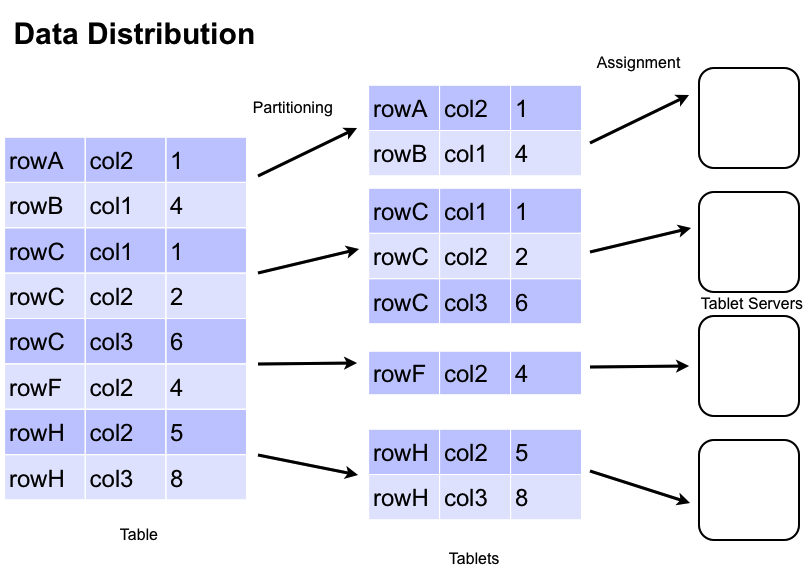
\includegraphics[scale=0.4]{images/data_distribution.png}
\end{center}

\section{Tablet Service}


When a write arrives at a TabletServer it is written to a Write-Ahead Log and
then inserted into a sorted data structure in memory called a MemTable. When the
MemTable reaches a certain size the TabletServer writes out the sorted key-value
pairs to a file in HDFS called Indexed Sequential Access Method (ISAM)
file. This process is called a minor compaction.  A new MemTable is then created
and the fact of the compaction is recorded in the Write-Ahead Log.

When a request to read data arrives at a TabletServer, the TabletServer does a
binary search across the MemTable as well as the in-memory indexes associated
with each ISAM file to find the relevant values. If clients are performing a
scan, several key-value pairs are returned to the client in order from the
MemTable and the set of ISAM files by performing a merge-sort as they are read.

\section{Compactions}

In order to manage the number of files per tablet, periodically the TabletServer
performs Major Compactions of files within a tablet, in which some set of ISAM
files are combined into one file. The previous files will eventually be removed
by the Garbage Collector. This also provides an opportunity to permanently
remove deleted key-value pairs by omitting key-value pairs suppressed by a
delete entry when the new file is created.

\section{Splitting}

When a table is created it has one tablet.  As the table grows its initial
tablet eventually splits into two tablets.   Its likely that one of these
tablets will migrate to another tablet server.  As the table continues to grow,
its tablets will continue to split and be migrated.  The decision to
automatically split a tablet is based on the size of a tablets files.   The
size threshold at which a tablet splits is configurable per table.  In addition
to automatic splitting, a user can manually add split points to a table to
create new tablets.  Manually splitting a new table can parallelize reads and
writes giving better initial performance without waiting for automatic
splitting.

As data is deleted from a table, tablets may shrink.  Over time this can lead
to small or empty tablets.   To deal with this, merging of tablets was
introduced in Accumulo 1.4.  This is discussed in more detail later.

\section{Fault-Tolerance}

If a TabletServer fails, the Master detects it and automatically reassigns the tablets
assigned from the failed server to other servers. Any key-value pairs that were in
memory at the time the TabletServer fails are automatically reapplied from the Write-Ahead
Log to prevent any loss of data.

The Master will coordinate the copying of write-ahead logs to HDFS so the logs
are available to all tablet servers. To make recovery efficient, the updates
within a log are grouped by tablet.  TabletServers can quickly apply the
mutations from the sorted logs that are destined for the tablets they have now
been assigned.

TabletServer failures are noted on the Master's monitor page, accessible via\\
\mbox{http://master-address:50095/monitor}.

\begin{center}
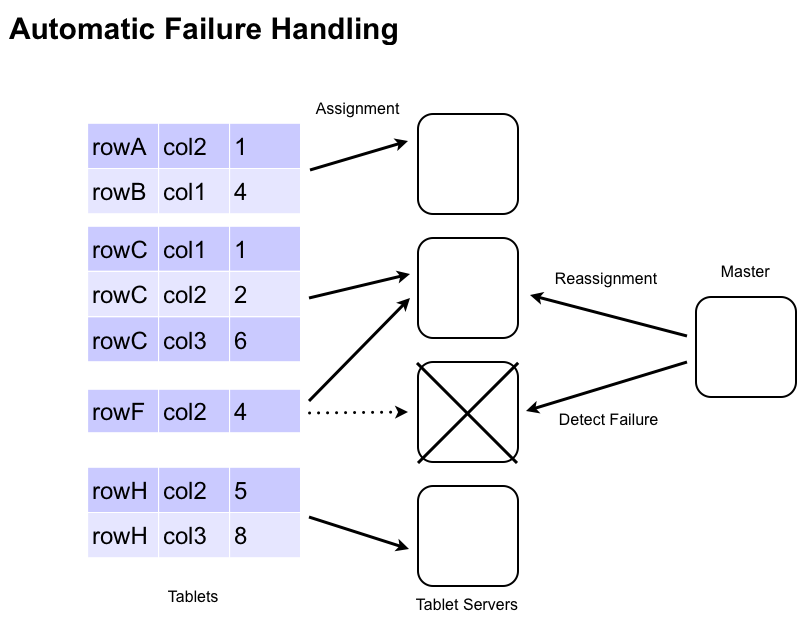
\includegraphics[scale=0.4]{images/failure_handling.png}
\end{center}

